\documentclass[11pt]{article}
\usepackage{latexsym}
\usepackage{amsmath}
\usepackage{amssymb}
\usepackage{amsthm}
\usepackage{epsfig}
\usepackage[tight]{subfigure}

\usepackage{amsmath}

\DeclareMathOperator*{\minimize}{min}
\DeclareMathOperator*{\maximize}{max}

\usepackage{algorithm}
 %on linux you may need to run sudo apt-get install texlive-full to install algorithm.sys
\usepackage{algorithmic}

\usepackage{verbatim}

\newcommand{\handout}[5]{
  \noindent
  \begin{center}
  \framebox{
    \vbox{
      \hbox to 5.78in { {#1} \hfill #2 }
      \vspace{4mm}
      \hbox to 5.78in { {\Large \hfill #5  \hfill} }
      \vspace{2mm}
      \hbox to 5.78in { {\em #3 \hfill #4} }
    }
  }
  \end{center}
  \vspace*{4mm}
}

\newcommand{\lecture}[5]{\handout{#1}{#2}{#3}{#4}{#5}}
\newcommand{\collision}[0]{\mathrm{collision}}
\newcommand{\nocollision}[0]{\overline{\collision}}

\newcommand*{\QED}{\hfill\ensuremath{\square}}

\newtheorem{theorem}{Theorem}
\newtheorem{corollary}[theorem]{Corollary}
\newtheorem{lemma}[theorem]{Lemma}
\newtheorem{observation}[theorem]{Observation}
\newtheorem{proposition}[theorem]{Proposition}
\newtheorem{definition}[theorem]{Definition}
\newtheorem{claim}[theorem]{Claim}
\newtheorem{fact}[theorem]{Fact}
\newtheorem{assumption}[theorem]{Assumption}
\newtheorem{note}[theorem]{Note}

% 1-inch margins, from fullpage.sty by H.Partl, Version 2, Dec. 15, 1988.
\topmargin 0pt
\advance \topmargin by -\headheight
\advance \topmargin by -\headsep
\textheight 8.9in
\oddsidemargin 0pt
\evensidemargin \oddsidemargin
\marginparwidth 0.5in
\textwidth 6.5in

\parindent 0in
\parskip 1.5ex
%\renewcommand{\baselinestretch}{1.25}

\begin{document}

\lecture{Statistical Techniques in Robotics (16-831, S22)}{Lecture \#10
  (Monday, February 21)}{Lecturer: Kris Kitani}{Scribe: Roshini Rajesh Kannan}{Support Vector Machine}

\section{Review}
In the course so far, we have seen Prediction with Expert Advice (PWEA) algorithms that had the characteristics of one-shot, instructive and exhaustive data. Later we moved to Online Linear Classification that included perceptron and winnowing algorithms. From there we moved to Online Convex Optimization problems that included Follow the Leader, Follow the regularized leader and we also connected it to Online Mirror Descent. Now in this lecture, we will be seeing (Online) Supervised Learning and how some supervised learning algorithms like Support Vector Machine can be solved using online learning algorithms. 

%This section serves as a review of the previous lecture and any other context required to frame the content of the current lecture. 

%You may format the scribes in any way you like, aside from changing font style, size and page format. Please use subsections and paragraphs to increase the readability of your notes.

%Length requirement 1-2 pages.
        
\subsection{Gradient descent}
Last lecture we saw the concept of Gradient Descent and Stochastic Gradient Descent. It further explained how Online Gradient Descent is a special case of Online Mirror Descent (OMD). In the review will cover Gradient Descent and its links with OMD.
Gradient Descent is an approach for minimizing differentiable (or non-differentiable in case of sub gradient descent) convex functions with regularization as an added constraint. From gradient descent we get updates in the form of  
\begin{equation}\label{grad_descent}
 \mathbf{w}=\mathbf{w}^{(t)}-\eta\nabla f(\mathbf{w}^{(t)})
 \end{equation}
 
This form of the parameter update is a result of:
\begin{enumerate}
    \item A quadratic approximation of the loss function f
    \item Linear loss function f with quadratic regularization
    \item Quadratic loss function with linear constraints
\end{enumerate}

 \begin{figure}[h!]
    \centering
  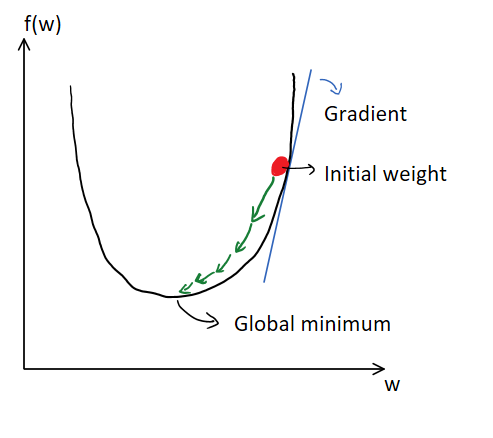
\includegraphics[scale=0.7]{fig7.PNG}
  \caption{Geometric representation of gradient descent}
  \label{fig:gd}
\end{figure}
The figure \ref{fig:gd} shows the geometric interpretation of gradient descent. We can approximate this to speed up the computation through Stochastic Gradient Descent(SGD) or Online Gradient Descent(OGD)
\subsection{Online Gradient Descent(OGD)}
Online Mirror Descent is often used to solve optimization problems that contain a linear loss function $f(\mathbf{w})$ and a quadratic regularization $\psi(\mathbf{w})$. In case of OGD, we can write them as:\begin{equation}\label{OMD}
\psi(\mathbf{w}) = \frac{1}{2\eta}||\mathbf{w}||_{2}^{2} \text{  and } f(w) = \langle \mathbf{w},\mathbf{\theta} \rangle
 \end{equation}
\[\]
Where $\mathbf\theta$ is the parameter for dual space. From equation \ref{OMD} we can see that $f(\mathbf{w})$ is linear and $\psi(\mathbf{w})$ is quadratic for OGD. Further when we solve for optimal parameter to minimize the convex function, we notice that $\mathbf{w}_{n} = \eta\mathbf{\theta}$.
Hence the mirror function for OGD is $g(\mathbf{\theta}) = \eta\mathbf{\theta}$. Therefore OGD is OMD with a linear loss and quadratic regularization (or quadratic loss with linear constraints).
\section{Summary}
\subsection{Online learning and Supervised Learning}
\normalfont
Online learning mainly has 2 steps: Update and Prediction. After the prediction, it calculates the loss and repeats the same process again. In supervised learning, the two steps happen distinctly and there is no continuous interaction between both. The parameters are fixed before testing and are not updated regularly. In figure \ref{fig:online}, When we look closely, we can see that, the learning algorithm in the training part of supervised algorithm can be an online learning algorithm. In this way, we see that some supervised learning algorithms can be solved using online algorithms. Now, let us see how online learning algorithms are hidden in supervised learning algorithms like SVM.
\begin{figure}[h!]
    \centering
  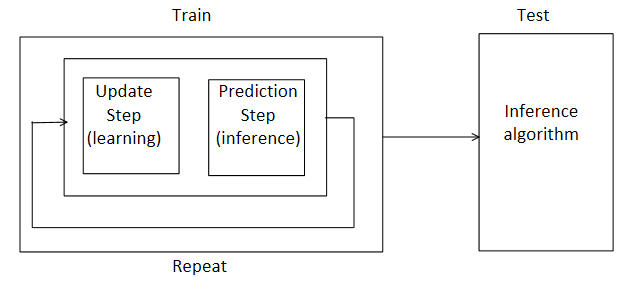
\includegraphics[scale=0.7]{fig1.PNG}
  \caption{Online learning Vs. Supervised Learning}
  \label{fig:online}
\end{figure}
\subsection{Hyperplanes}
\definition{\normalfont\textbf{Hyperplanes} Is a subspace with a dimension one less than the dimension of the space in which it is present.}\\\normalfont
Before moving ahead to SVM, we need to understand the concept of hyperplanes to know about its geometry.
\subsubsection{Hyperplanes in 2D}
Hyperplanes are lines in 2-D and can be written as dot product plus a bias. 
\begin{equation}\label{hp1}
    \mathbf{w}\cdot \mathbf{x}+b=0
\end{equation}
The distance between a point $(x_0,y_0)$ and line can be given by the equation 
\begin{equation}\label{hp2}
    \frac{|\mathbf{w}\cdot \mathbf{x}+b|}{||\mathbf{w}||}
\end{equation}
For the distance between the origin and line, we have to substitute the value of $(x_0,y_0)$ as $(0,0)$:
\begin{equation}\label{norm}
     \frac{b}{||\mathbf{w}||}
\end{equation}  From equation \ref{norm} we get the distance from origin to be $\frac{b}{||\mathbf{w}||}$ also shown in figure \ref{fig:fig2}.
\begin{figure}[h!]
    \centering
  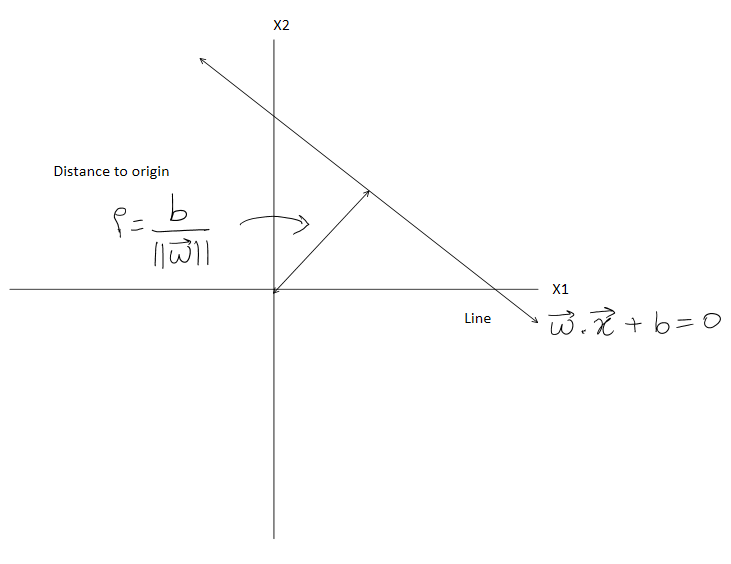
\includegraphics[scale=0.7]{fig2.PNG}
  \caption{Distance from a line to origin}
  \label{fig:fig2}
\end{figure}
\\Similarly, we try to find the distance between two lines, where line 1 is $\mathbf{w}.\mathbf{x}+b=0$ and line 2 is $\mathbf{w}.\mathbf{x}+b=-1$. Then the distance of line 1 to origin would be $\frac{b}{||\mathbf{w}||}$ and the distance of line 2 to origin would be $\frac{b+1}{||\mathbf{w}||}$. The difference between these distances would give the distance between the lines which is $\frac{1}{||\mathbf{w}||}$.



\subsubsection{Hyperplanes in 3D}
\begin{figure}[h!]
    \centering
  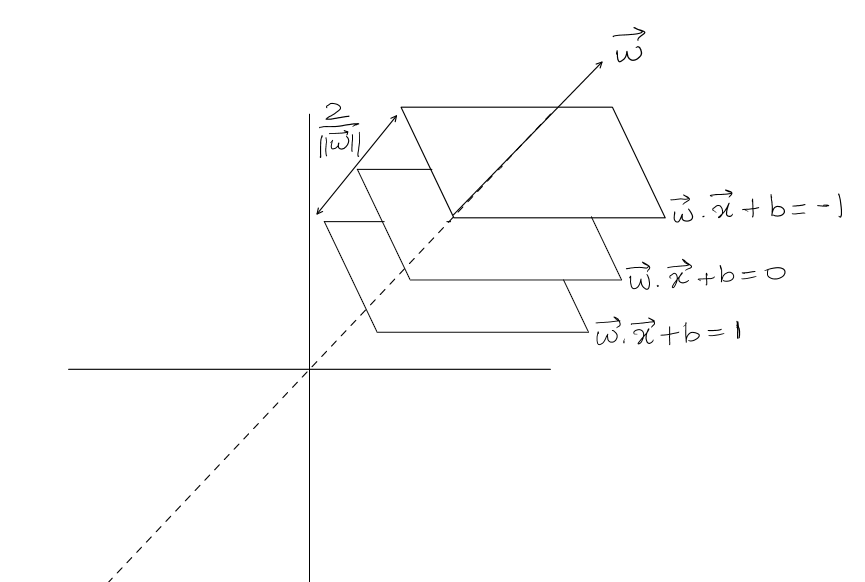
\includegraphics[scale=0.7]{fig3.PNG}
  \caption{Distance between 2 hyperplanes}
  \label{fig:dplane}
\end{figure}
The hyperplanes in 3D also have an equation of $\mathbf{w}\cdot\mathbf{x}+b=0$, where the dimensions of the \textbf{w} and \textbf{x} vectors without bias is the dimension of the plane. Consider we have 3 planes $\mathbf{w}\cdot\mathbf{x}+b=0$, $\mathbf{w}\cdot\mathbf{x}+b=-1$ and $\mathbf{w}\cdot\mathbf{x}+b=1$ as shown in figure \ref{fig:dplane}. Then the distance between each of the outer planes to the centre plane is $\frac{1}{||\mathbf{w}||}$. And the distance between the two outer planes is $\frac{2}{||\mathbf{w}||}$


\subsection{Support Vector Machine}
When we try to find out the best hyperplane for a binary classification case, we might intuitively say it as the one that has the highest margin, i.e, the one which is farthest from all the interior points. In figure \ref{fig:SV1}, the highlighted points are the ones closest to the planes and they are called the support vectors. So mathematically our goal is to find a $\mathbf{w}$ that maximizes the distance between the parallel planes which is $\frac{2}{||\mathbf{w}||}$ as shown. 
\begin{figure}[h!]
    \centering
  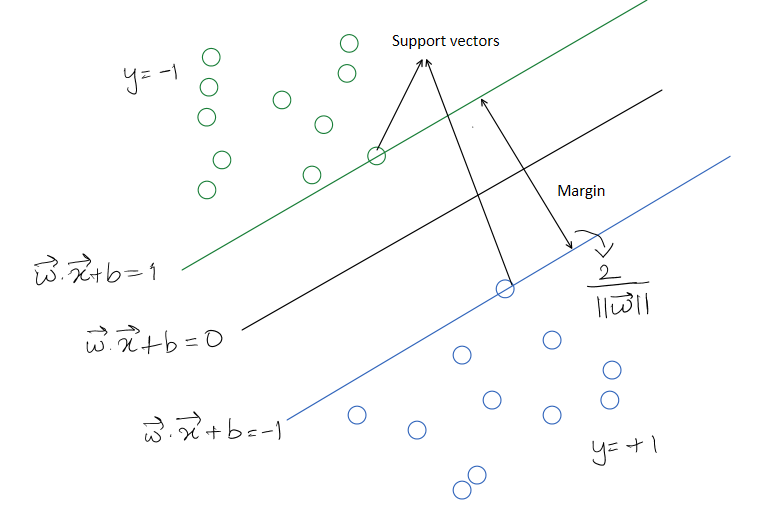
\includegraphics[scale=0.7]{fig4.PNG}
  \caption{Support Vector}
  \label{fig:SV1}
\end{figure}
\\
\\Apart from maximum margin, we also need to classify the points correctly, hence, there are 2 constraints added to make the goal more specific.
\begin{equation}\label{max}
    \text{max }\frac{2}{||\mathbf{w}||} \text{ subject to } \mathbf{w}\cdot\mathbf{x}_i+b\geq +1 \text{ if } y_i=+1 \text{ and } \mathbf{w}\cdot\mathbf{x}_i+b\leq -1 \text{ if } y_i=-1
\end{equation}

The margin here need not necessarily be 1, it can be any constant value. The above maximization problem can also be written as an equivalent minimization problem as:
\begin{equation}\label{min}
    \text{min }||\mathbf{w}||^2 \text{ subject to the condition } y_i(\mathbf{w}\cdot\mathbf{x}_{i}+b)\geq1 \text{ for i=1,...,N}
\end{equation}
Finding the arg min $\mathbf{w}$ that minimizes $||\mathbf{w}||$ will be same as the $\mathbf{w}$ that minimizes $||\mathbf{w}||^2$. Hence, we have equation {\ref{min}} to add more penalty on w. The above equation is the primal formulation of a linear SVM. Since the constraints are satisfied, we call this the Hard SVM.
\subsection{Soft margin SVM}
Equation \ref{min} in the previous section is the constraint for the objective function of SVM and this is called the hard constraint. We might not be able to satisfy this constraint when the data is too noisy or if it is not linearly separable. This is the case of soft-SVM. If we try to find the best hyperplane in soft SVM that doesn't make any mistake, then the margin might be too narrow. Intuitively it might be better to allowing some misclassifications that might make the model more robust. \\ \\
By allowing few mistakes we can get a bigger margin. To allow some misclassifications we modify the constraint by adding a slack variable $\xi_i$. 
\begin{figure}[h!]
    \centering
  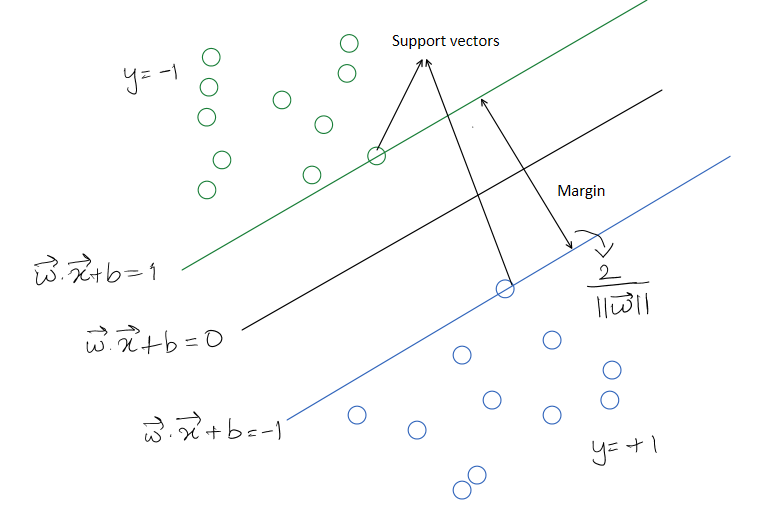
\includegraphics[scale=0.7]{fig4.PNG}
  \caption{Slack Variable}
  \label{fig:SV}
\end{figure}
Geometrically the slack variable is the distance of the point from the margin on the correct side the point has to be as shown in figure \ref{fig:SV}. The slack variable is always positive and we want it to be closer to zero so that the misclassified point is closer to its correct classification side. 
\\The objective for soft margin is \begin{equation}
    \label{min2}
    \min_{\mathbf{w},\xi}||\mathbf{w}||^2 + C\sum_i \xi_i
\end{equation} and it is subject to \begin{equation}
    \label{min2_constraints} y_i(\mathbf{w}^{T}\mathbf{x}_i+b)\geq 1-\xi_i \text{ for i=1,2,...,N}
\end{equation}
In equation \ref{min2}, C is a regularization parameter. If C is close to zero, then constraints are ignored and we get a larger margin. When C is close to infinity, there is huge penalty and the margin is small. Let us now solve this problem. \\From equation \ref{min2_constraints} we get,
\begin{equation}
    \label{slack}
1- y_i(\mathbf{w}^{T}\mathbf{x}_i+b)\leq \xi_i
\end{equation}
 By substituting this to the objective function we get,
 \begin{equation}
    \label{slack}\min_\mathbf{w}(\frac{\lambda}{2}||\mathbf{w}||^2+\frac{1}{N}\sum_{n=1}^{N}1-y_n\mathbf{w}^T\mathbf{x}_n)
    \end{equation}
  The drawback with this equation is very large negative value for some correctly classified points overpowers positive values for mistaken points. In order to correct this, we want to penalize for mistakes, weakly correct and ignore ‘very correct’ data.
To achieve this, we replace the term $1-y_n\mathbf{w}^T\mathbf{x}_n$ with the hinge loss max\{0,$1-y_n\mathbf{w}^T\mathbf{x}_n$\}. The function now becomes,\begin{equation}
    \label{function}
    \min_\mathbf{w}(\frac{\lambda}{2}||\mathbf{w}||^2+\frac{1}{N}\sum_{n=1}^{N}max\{0,1-y_n\mathbf{w}^T\mathbf{x}_n\} 
    \end{equation}
where the first term is the regularisation term and the second term is the loss function. This is a convex function and online mirror descent due to a piecewise linear hinge loss and quadratic regularisation function. This function is not differentiable due to max function in hinge loss. Since it is a convex non-differentiable function, we optimize it using the Online Sub-Gradient Descent.
\begin{figure}[h!]
    \centering
  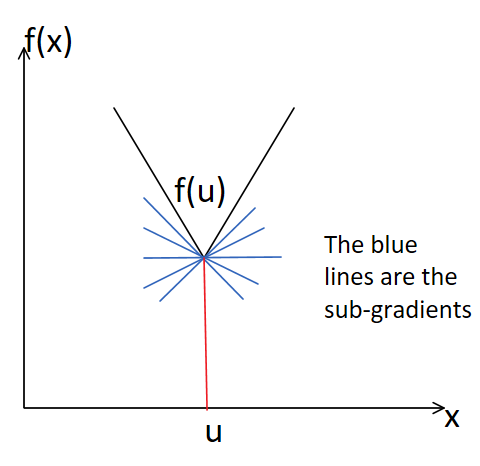
\includegraphics[scale=0.7]{fig6.PNG}
  \caption{Sub-gradients}
  \label{fig:SG}
\end{figure}
In figure \ref{fig:SG} we can see that when a convex function is non-differentiable, as it has many lines that lower bound the function $f(\mathbf{x})$ at $x=u$. These are the sub-gradients. To optimize our objective function, we will have to get the sub-gradients of the hinge loss. There are many possible sub-gradients, but we select the following two:
\begin{equation}
    \label{function}\mathbf{z}_n=\begin{cases}
0 \text{ if } y_{n}\mathbf{w}^{T}\mathbf{x}_n\geq 1
\\-y_{n}\mathbf{x}_{n} \text{ otherwise}

\end{cases}
\end{equation}

\\The following is the algorithm for soft SVM:
\begin{algorithm}[H]
\caption{Soft SVM}
\label{algo:rwma}
\begin{algorithmic}[1]
\STATE $\textbf{$\theta$}^{(0)} \leftarrow $0 \in{\mathbb{R}^{(N)}}$ \hfill $\triangleright$ Theta initialization
\FOR{$t=1,\;\cdots,\;T$}

\STATE $y_d,\mathbf{x}_d\sim$ \textsc{D} \hfill $\triangleright$ Receive training data
\STATE $\mathbf{\theta}^{(t)}=\mathbf{\theta}_{(t-1)}+y_{d}\mathbf{x}_{d} . \mathbf{1}[y_{d}(\mathbf{w}^{(t)}.x^{(y)})]<1$ \hfill $\triangleright$ Dual parameter update
\STATE $\mathbf{w}^{(t+1)}\leftarrow \frac{1}{\lambda(t+1)}\mathbf{\theta^{(t)}} \hfill $\triangleright$ Weight update
\ENDFOR
\end{algorithmic}
\end{algorithm}


\subsection{Comparison with Perceptron algorithm}
\begin{algorithm}[H]
\caption{Perceptron Algorithm}
\label{algo:perceptron}
\begin{algorithmic}[1]
\STATE $\textbf{$w$}^{(0)} \leftarrow $0 $ \hfill $\triangleright$ Weight initialization
\FOR{$t=1,\;\cdots,\;T$}

\STATE RECEIVE$(\mathbf{x}^{(t)}y^{(t)})$\hfill \triangleright$ Receive training data
\STATE $\mathbf{\theta}^{(t)}=\mathbf{\theta}_{(t-1)}+y^{(t)}\mathbf{x}^{(t)} . \mathbf{1}[y^{(t)}\langle\mathbf{w}^{(t)},x^{(t)}\rangle<0]$ \hfill $\triangleright$ Dual parameter update
\STATE $\mathbf{w}^{(t+1)}={\mathbf{\theta}^{(t)}} \hfill $\triangleright$ Mirror projection
\ENDFOR
\end{algorithmic}
\end{algorithm}

Both SVM and Perceptron have similar dual parameter update. SVM uses soft margin whereas, perceptron uses no margin. They both have a similar mirror function. Both have piecewise linear hinge loss and a quadratic regularisation.


\pagebreak

\section{Appendix}
\subsection{Multi-class SVM}
Handling multiclass data with SVMs is still an active area of research. Methods involve creating multiple SVMs that compare feature vectors among themselves by using various techniques such as one-versus-Rest (OVR) or one-versus-one (OVO). For k classes, the OVR method trains k classifiers so that each class discriminates against the remaining k-1 classes. OVO creates one binary classification problem for all possible pairings of classes, so it requires $\frac{k(k-1)}{2}$ classifiers\cite{bhattacharyya_2020}. After constructing the number of required binary classifiers for either the OVR or OVO methods, the algorithm classifies a new object according the majority vote among the set of classifiers.
\subsection{Advantages of SVM}
\begin{enumerate}
    \item Can easily accommodate data with large feature dimensions 
    \item Require fewer computational resources for both training and classification\cite{pisner2020support}
    \item Less likely to overfit
\end{enumerate}
\subsection{Lagrangian Dual Form}
The primal quadratic form can become hard to solve with large datasets because the optimization space considers the dot product of w and all the training. Hence, we use a dual form based on Lagrangian multipliers\cite{bridgelall2022tutorial}. Some benefits of the dual form are a reduction of computational resources and using Kernel functions to find suitable hyperplanes that can separate non-linearly separable data. The dual problem requires learning only the number of support vectors. \\Constructing the dual form involves constructing the Lagrange, by
combining both the objective function $f(w)$ and the equality constraint $g(w)$ such that the Lagrangian function $L(w) = f(w) – \lambda g(w)$ with $\lambda$ being the so-called Lagrangian multiplier.
Hence, the objective function 
\[f=\frac{1}{2}||w||^2\] and constraint \[ y_i(w\cdot x_i+b)-1=0\] gives the dual form of
\begin{equation}
    \label{function}L(\alpha,w,b)=\frac{1}{2}||w||^2-\sum_1\alpha_i[(y_i(w\cdot x_i+b)-1]
    \end{equation}
\\The maximum (or minimum) solutions of the Lagrangian that satisfies the constraints are where the gradient is zero 
%This section provides any relevant background material that was not covered in the lectures, but was found to be useful for understanding the material. 
%For example, derivations, theory underlying techniques employed, etc. 

%Additionally, this section can summarizes applications or extensions of these techniques found in the literature. 
\pagebreak

%Include your references here. Please cite any resources you found useful.	
%Populate the refs.bib file or list your references manually. Be consistent in formatting!
{
\bibliography{refs}
\bibliographystyle{abbrv}
}
\end{document} % Done!


